\documentclass[10pt,twocolumn,letterpaper]{article}

\usepackage{iccv_rebuttal}
\usepackage{times}
\usepackage{epsfig}
\usepackage{graphicx}
\usepackage{amsmath}
\usepackage{amssymb}

% Include other packages here, before hyperref.

% If you comment hyperref and then uncomment it, you should delete
% egpaper.aux before re-running latex.  (Or just hit 'q' on the first latex
% run, let it finish, and you should be clear).
\usepackage[pagebackref=true,breaklinks=true,letterpaper=true,colorlinks,bookmarks=false]{hyperref}

%%%%%%%%% PAPER ID  - PLEASE UPDATE
\def\iccvPaperID{8604} % *** Enter the ICCV Paper ID here
\def\httilde{\mbox{\tt\raisebox{-.5ex}{\symbol{126}}}}

\begin{document}

%%%%%%%%% TITLE - PLEASE UPDATE
\title{STANLEY: Stochastic Gradient Anisotropic Langevin Dynamics for Learning Energy-Based Models}  % **** Enter the paper title here

\maketitle
\thispagestyle{empty}


%%%%%%%%% BODY TEXT - ENTER YOUR RESPONSE BELOW

We would like to thank the three reviewers for their feedback. 
Upon acceptance, we will include in the final version \emph{{\sf (a)} a clearer presentation of the algorithms} and \emph{{\sf (b)} additional experiments}. 


We would like to address common concerns shared by the reviewers, noted R1, R2 and R3 for conciseness.

\noindent  \textbf{-- Notations (R1/R2):}
Upon acceptance, the revised paper will fix and include more comprehensive notations, particularly used throughout the theory section of our contribution.
The algorithm typos, in line 6, has been fixed (the stepsize does follow the EBM iteration index and not the MCMC iterations). We thank the reviewers for having pointed it out.

\noindent \textbf{-- Longer training procedures (R1/R2):}
Longer training procedure is doable, yet we want to stress of the fundamental aspect of our contribution. We develop STANLey in order to more efficiently sample from the Gibbs potential. Hence, our goal is not to reach an optimal and high resolution generated image, but rather to decrease the number of kernel transitions need at each EBM iteration in order to obtain relatively good samples.
Drastically reducing this number would have a great impact on the energy consumption and speed of the whole training process.


\noindent \textbf{-- Additional numerical experiments (R1/R2/R3):}

\textit{More baselines:}


\begin{figure}
\begin{center}
\mbox{\hspace{-0.2in}
        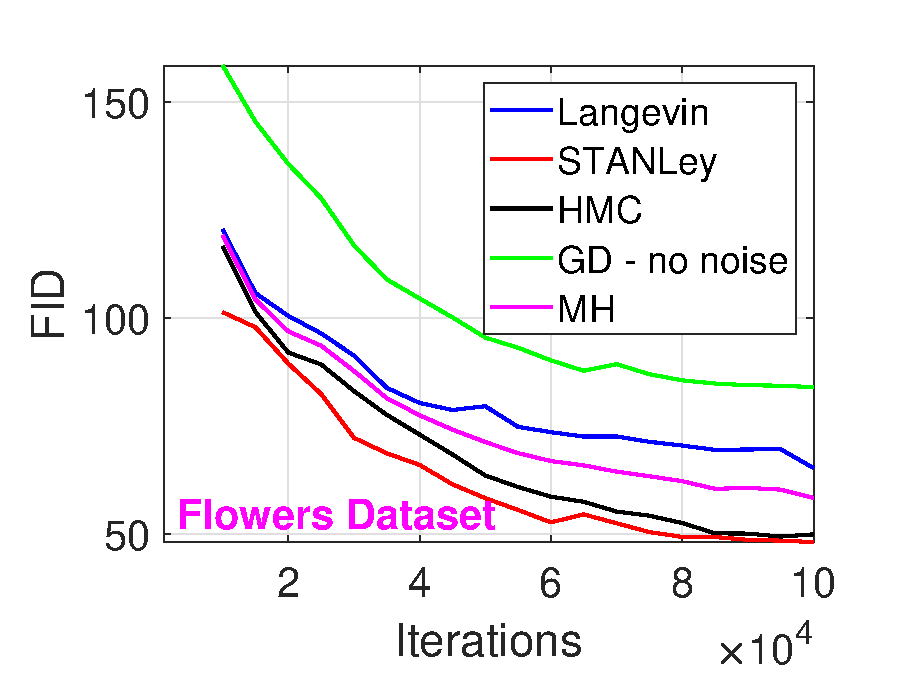
\includegraphics[width=1.9in]{figs/fid_flowersmore.eps} \hspace{-0.2in}
        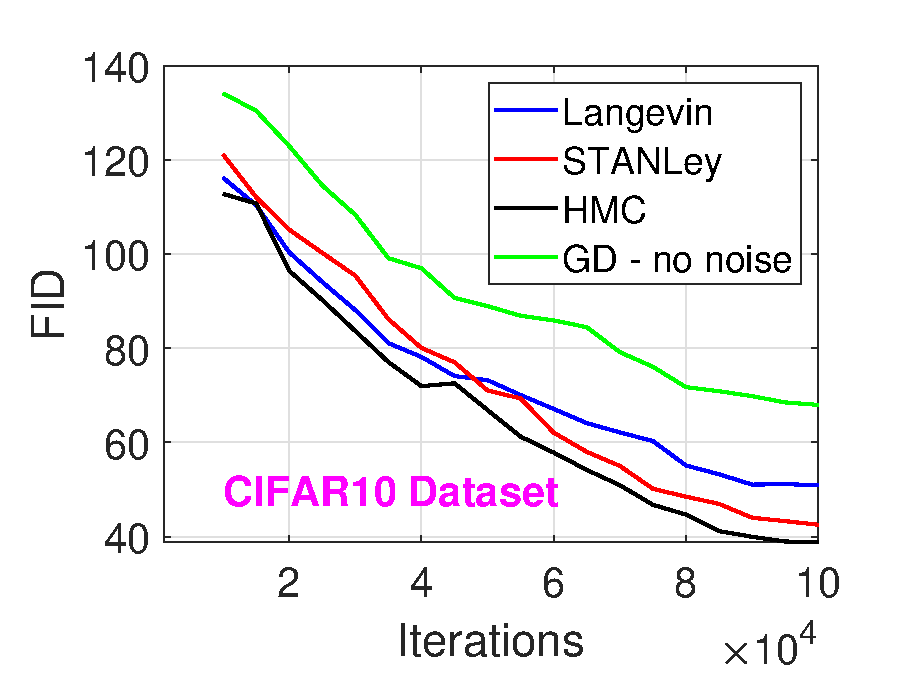
\includegraphics[width=1.9in]{figs/fid_cifarmore.eps}
        
}
\end{center}
	\caption{(FID values per method against 100k iterations elapsed). Left: Oxford Flowers dataset. Right: CIFAR-10 dataset.}
	\label{fig:fidall}
\end{figure}

\begin{figure}
\begin{center}
    \mbox{
        \includegraphics[width=1.65in]{figs/cifaranila}
        \includegraphics[width=1.65in]{figs/mh_x_q_099900}
        }\vspace{0.05in}
            \mbox{
                \includegraphics[width=1.65in]{figs/hmc_x_q_099900}
                        \includegraphics[width=1.65in]{figs/gd_x_q_099900}
        }
\end{center}
\caption{(CIFAR Dataset). 1: STANLey 2: MH. 3: HMC 4: GD without noiseAfter 100k iterations.}
	\label{fig:cifar}
\end{figure}

\noindent \textbf{-- Originality of our contributions (R1/R2/R3):}



% {\small
% \bibliographystyle{ieee}
% \bibliography{refrebuttal}
% }

\end{document}
